% Options for packages loaded elsewhere
\PassOptionsToPackage{unicode}{hyperref}
\PassOptionsToPackage{hyphens}{url}
%
\documentclass[
]{article}
\usepackage{amsmath,amssymb}
\usepackage{iftex}
\ifPDFTeX
  \usepackage[T1]{fontenc}
  \usepackage[utf8]{inputenc}
  \usepackage{textcomp} % provide euro and other symbols
\else % if luatex or xetex
  \usepackage{unicode-math} % this also loads fontspec
  \defaultfontfeatures{Scale=MatchLowercase}
  \defaultfontfeatures[\rmfamily]{Ligatures=TeX,Scale=1}
\fi
\usepackage{lmodern}
\ifPDFTeX\else
  % xetex/luatex font selection
\fi
% Use upquote if available, for straight quotes in verbatim environments
\IfFileExists{upquote.sty}{\usepackage{upquote}}{}
\IfFileExists{microtype.sty}{% use microtype if available
  \usepackage[]{microtype}
  \UseMicrotypeSet[protrusion]{basicmath} % disable protrusion for tt fonts
}{}
\makeatletter
\@ifundefined{KOMAClassName}{% if non-KOMA class
  \IfFileExists{parskip.sty}{%
    \usepackage{parskip}
  }{% else
    \setlength{\parindent}{0pt}
    \setlength{\parskip}{6pt plus 2pt minus 1pt}}
}{% if KOMA class
  \KOMAoptions{parskip=half}}
\makeatother
\usepackage{xcolor}
\usepackage[margin=1in]{geometry}
\usepackage{graphicx}
\makeatletter
\def\maxwidth{\ifdim\Gin@nat@width>\linewidth\linewidth\else\Gin@nat@width\fi}
\def\maxheight{\ifdim\Gin@nat@height>\textheight\textheight\else\Gin@nat@height\fi}
\makeatother
% Scale images if necessary, so that they will not overflow the page
% margins by default, and it is still possible to overwrite the defaults
% using explicit options in \includegraphics[width, height, ...]{}
\setkeys{Gin}{width=\maxwidth,height=\maxheight,keepaspectratio}
% Set default figure placement to htbp
\makeatletter
\def\fps@figure{htbp}
\makeatother
\setlength{\emergencystretch}{3em} % prevent overfull lines
\providecommand{\tightlist}{%
  \setlength{\itemsep}{0pt}\setlength{\parskip}{0pt}}
\setcounter{secnumdepth}{-\maxdimen} % remove section numbering
\usepackage{booktabs}
\usepackage{wrapfig}
\usepackage{graphicx}
\usepackage{amssymb}
\usepackage{tikz}
\usepackage{amsmath}
\usepackage{color}
\usepackage{subcaption}
\usepackage[font=footnotesize]{caption}
\usepackage[labelfont=bf,textfont=md]{caption}
\usepackage{titling}
\captionsetup[figure]{font=small}
                                          
\DeclareRobustCommand{\solidline}{\raisebox{2pt}{\tikz{\draw[thick](0,0) -- (0.5,0);}}}
\DeclareRobustCommand{\dashedline}{\raisebox{2pt}{\tikz{\draw[dashed, thick](0,0) -- (0.5,0);}}}                                          
\ifLuaTeX
  \usepackage{selnolig}  % disable illegal ligatures
\fi
\IfFileExists{bookmark.sty}{\usepackage{bookmark}}{\usepackage{hyperref}}
\IfFileExists{xurl.sty}{\usepackage{xurl}}{} % add URL line breaks if available
\urlstyle{same}
\hypersetup{
  hidelinks,
  pdfcreator={LaTeX via pandoc}}

\author{}
\date{\vspace{-2.5em}2024-05-15}

\begin{document}

\hypertarget{orion-star-ph-meter-cross-comparison-report}{%
\subsection{Orion Star pH Meter Cross Comparison
Report}\label{orion-star-ph-meter-cross-comparison-report}}

Sonya Havens\\
2024-06-04

\hypertarget{thermo-scientifictm-orion-startm-a211-benchtop-ph-meter}{%
\subsubsection{\texorpdfstring{Thermo Scientific\textsuperscript{TM}
Orion Star\(^TM^\) A211 Benchtop pH
Meter}{Thermo ScientificTM Orion Star\^{}TM\^{} A211 Benchtop pH Meter}}\label{thermo-scientifictm-orion-startm-a211-benchtop-ph-meter}}

The Thermo Scientific\textsuperscript{TM} Orion Star\textsuperscript{TM}
A211 Benchtop pH Meter was purchased from Fisher Scientific 23 March
2023 and included the following parts''

\begin{itemize}
\tightlist
\item
  Star A211 pH meter
\item
  8172BNWP ROSS Sure-Flow glass-body pH electrode
\item
  927007MD stainless steel ATC probe
\item
  810199 pH buffer kit
\item
  electrode stand
\item
  100-240V universal power adapter
\item
  computer cable
\end{itemize}

The Thermo Scientific\textsuperscript{TM} Orion Star\textsuperscript{TM}
A211 pH Meter was received 7 April 2023, installed on 12 June 2023, and
used to measure pH in samples collected from 12 June 2023 to 6 September
2023 (\emph{n} = 301) that were also measured on the Fisher Accumet
Benchtop pH Meter. Samples from the Environment and Climate Change
Canada Proficiency Testing study (ECCC-PT) were also analyzed on the
Shimadzu HIC-ESP and compared with ECCC-PT results. Instrument
performance data (e.g.~detection limits and reference samples) is also
provided.

\hypertarget{analytical-precision}{%
\subsubsection{Analytical precision}\label{analytical-precision}}

The analytical precision (\emph{Pr}), which is based on the residuals of
the standard buffers response along the calibration curve, is calculated
for each run using the measured response (mV) of standard buffers and
equations 1 through 3:

Equation 1. \(Pr = (y_d-b)/m\)

where \emph{b} is the y-intercept, \emph{m} is the slope, and
\emph{y\textsubscript{d}} is the signal detection limit, which is
calculated using equation 2.

Equation 2. \(y_d = 3s_y+b\)

where \emph{s\textsubscript{y}} is the residuals between the measured
response (mV) for each standard buffer and the calibration curve
predicted response (mV) for each standard concentration and is
calculated using equation 3.

Equation 3. \(s_y = √((∑d_i^2 )/(n-2))\)

where \emph{n} is the number of standards in the calibration curve, and
\emph{d\textsubscript{i}} is the difference between the measured
response (mV) for each standard buffer and the calibration curve
predicted response (mV) for each standard buffer.

The average analytical precision of pH measured on the Orion Star pH
meter and Fisher Accumet pH meter during the cross comparison period (14
March 2023 to 3 November 2023) were similar (0.05 ± 0.03, \emph{n} = 37
and 0.03 ± 0.03, \emph{n} = 87, respectively).

\hypertarget{duplicate-precision}{%
\subsubsection{Duplicate precision}\label{duplicate-precision}}

Sample duplicates are conducted every 15 to 20 samples. The average
relative percent difference (RPD) of duplicated samples, calculated
using equation 4, was \% (median = \%) and \% (median = \%) for samples
analysed on the Orion Star pH meter and on the Fisher Accumet pH meter,
respectively.

Equation 4. \(RPD = ((C_1-C_2)/((C_1+C_2)/2)) x 100\)

where \emph{C\textsubscript{1}} and \emph{C\textsubscript{2}} are the
concentrations of the two replicates.

\hypertarget{millivolt-stability-and-calibration-slope}{%
\subsubsection{Millivolt stability and calibration
slope}\label{millivolt-stability-and-calibration-slope}}

The millivolt (mV) values were stable throughout the cross comparison
study on the Orion Star pH meter, while the mV values were stable until
mid-September on the Fisher Accumet pH meter, at which point the mV
values of each pH buffer started to increase. The literature established
mV values for pH 4, 6, and 8 are 177, 59, and -59, respectively. The
average mV values for pH 4, 6, and 8 were 158 ± 5, 40 ± 5, and -76 ± 5
(\emph{n} = 37), respectively, on the Orion Star pH meter, which were
lower than literature established values by 19 ± 5, 19 ± 5, and 17 ± 5,
on average. The average mV values for pH 4, 6, and 8 on the Fisher
Accumet pH meter (186 ± 7, 69 ± 7, and -48 ± 7, respectively, \emph{n} =
87), were higher than established values by 9 ± 7, 10 ± 7, and 11 ± 7,
on average, but closer to literature established values than those
measured on the Orion Star pH meter.

\begin{figure}[h]
  \begin{subfigure}{0.48\textwidth}
  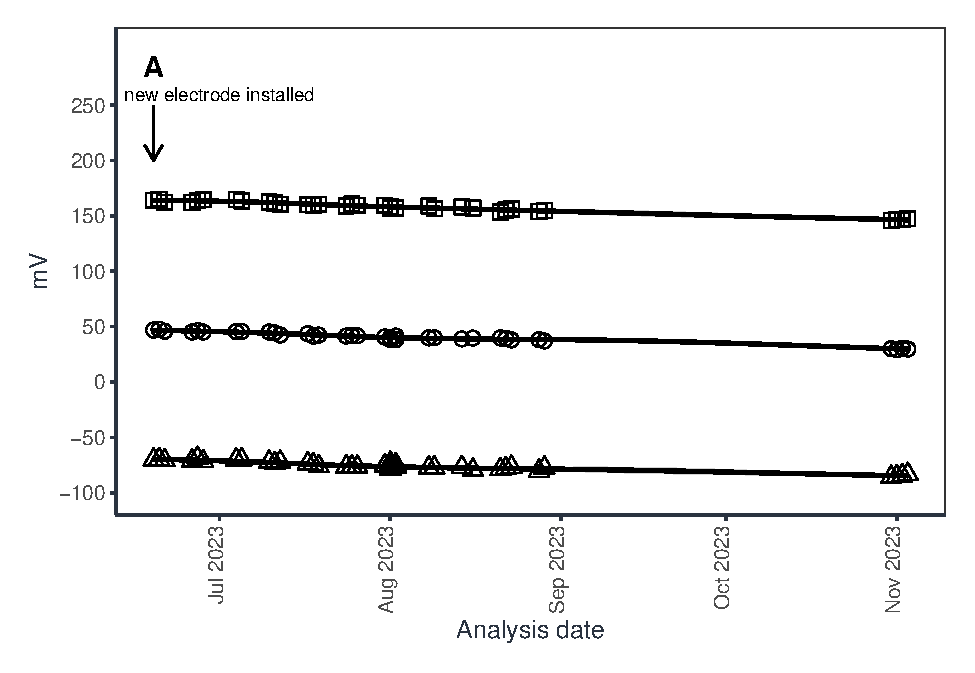
\includegraphics[]{orion_mV.pdf}
  \end{subfigure}%
  \begin{subfigure}{0.48\textwidth}
  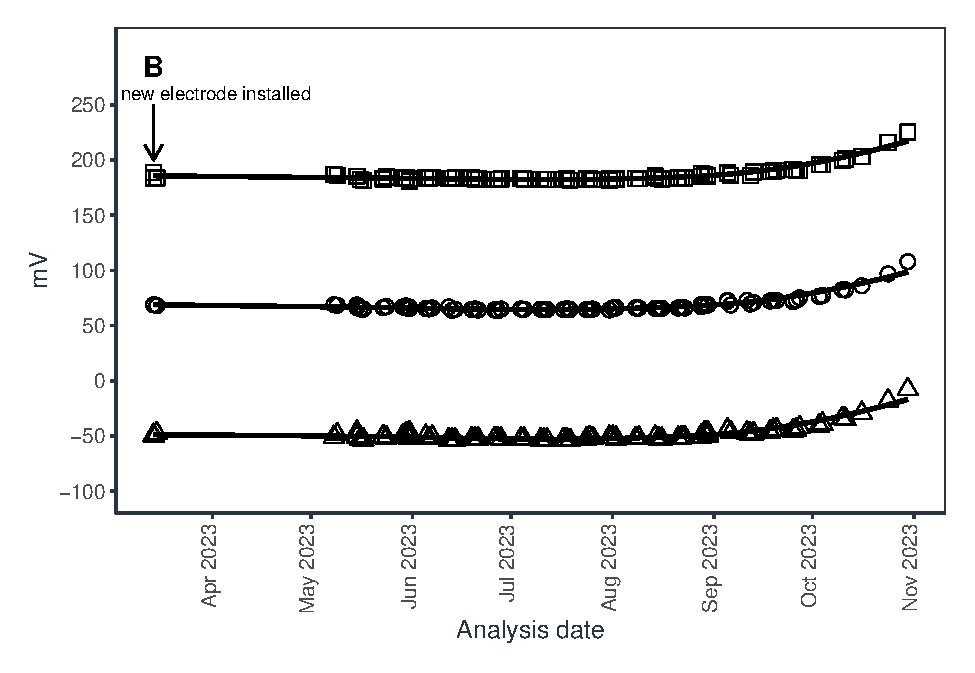
\includegraphics[]{fisher_mV.pdf}
  \end{subfigure}
\caption{pH meter signal response (mV) of pH 4 ($\square$), pH 6 ($\bigcirc$), and pH 8 ($\bigtriangleup$) buffers from 19 June 2023 to 3 November 2023 for the Orion Star pH meter and from 14 March 2023 to 30 October 2023 for the Fisher Accumet pH meter,}
\end{figure}

\begin{wrapfigure}[20]{r}{0.5\textwidth}
  \vspace{-0.5cm}
  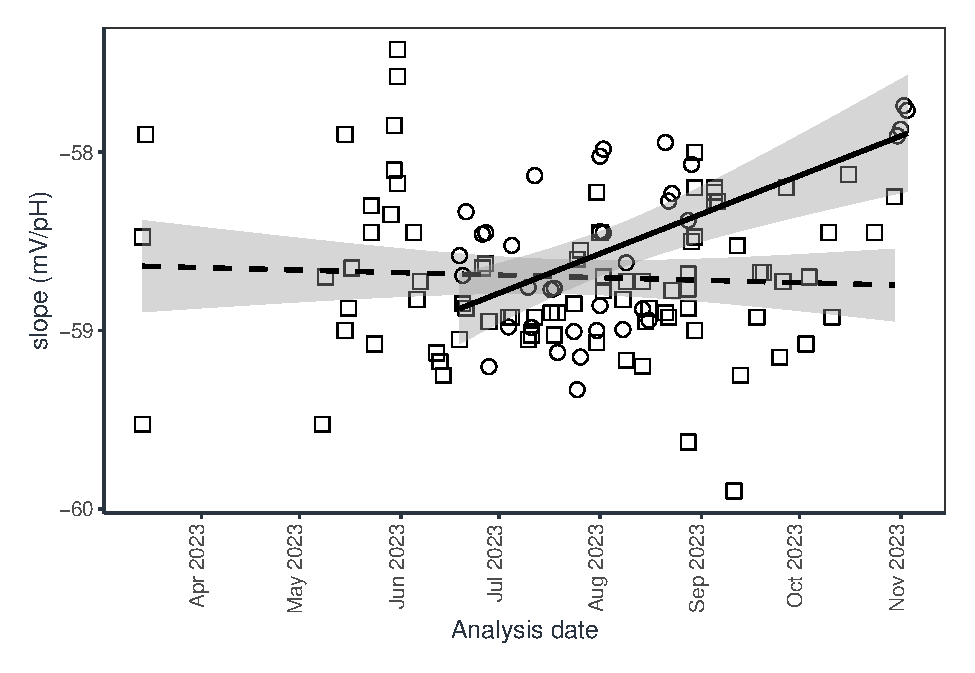
\includegraphics[width=0.5\textwidth]{mV_slope.pdf}
  \caption{Slope of pH meter calibrations of analytical runs on the Orion Star pH meter ($\bigcirc$, \protect\solidline, $\mbox{\textit{y}=0.0049}$$\textit{x}$$\mbox{-155}$, $\mbox{\textit{n}=40}$) from 19 June 2023 to 3 November 2023 and with the Fisher Accumet pH meter ($\square$, \protect\dashedline, $\mbox{\textit{y}=0.0003}$$\textit{x}$$\mbox{-65}$, $\mbox{\textit{n}=40}$) from 14 March 2023 to 30 October 2023.}
\end{wrapfigure}

Despite the stability of the mV values of pH buffers measured on the
Orion Star pH meter, the slope of the calibration curve decreased over
time (Figure 2). The slope started out near the ``ideal'' slope of -59
mV/pH, then slowly increased to \textasciitilde-58 mV/pH. The slope of
the calibration curve on the Fisher Accumet pH meter was stable over
time (Figure 2), however, there was more variability in the slope of the
Fisher Accumet calibrations (0.0008) than in the slope of the Orion Star
calibrations (0.0795). \pagebreak

\hypertarget{reference-samples}{%
\subsection{Reference samples}\label{reference-samples}}

\begin{wrapfigure}{r}{0.5\textwidth}
  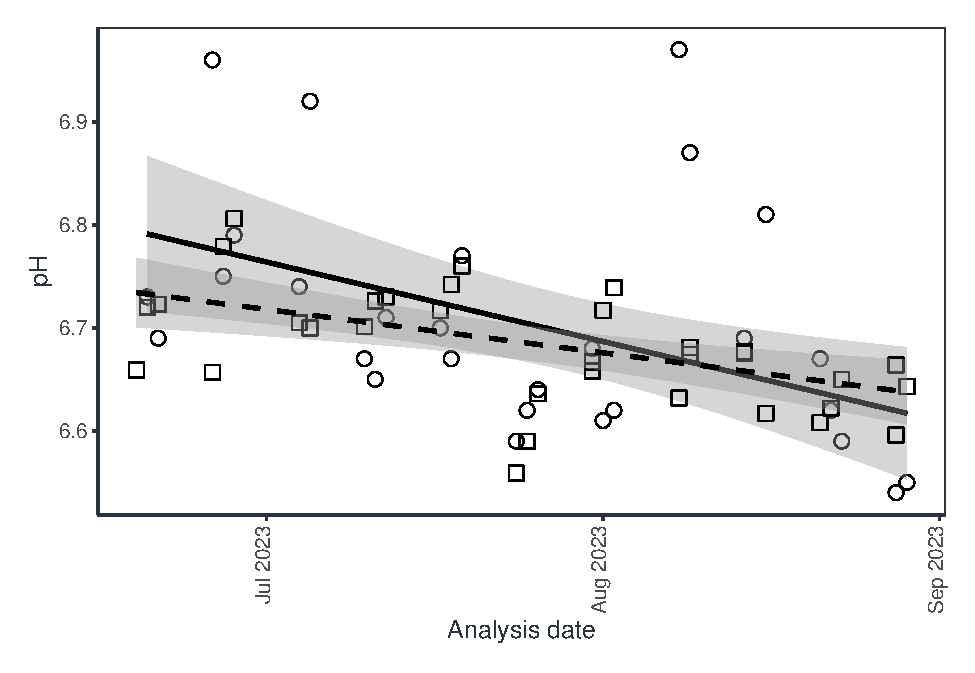
\includegraphics[width=0.5\textwidth]{ref_comparison_date.pdf}
  \caption{pH of reference sample measured with the Orion Star pH meter ($\bigcirc$, \protect\solidline, $\mbox{\textit{y}=-0.0025}$$\textit{x}$+$\mbox{55}$, $\mbox{\textit{n}=35}$) and with the Fisher Accumet pH meter ($\square$, \protect\dashedline, $\mbox{\textit{y}=-0.0014}$$\textit{x}$+$\mbox{33}$, $\mbox{\textit{n}=36}$) from June 2023 to September 2023.}
\end{wrapfigure}

A reference sample is included in each analytical run. The average pH
result of reference samples measured on the Orion Star and Fisher
Accumet were similar (6.71 ± 0.11, \emph{n} = 37 and 6.65 ± 0.12,
\emph{n} = 87, respectively). The pH of the reference sample, measured
by both the Orion Star and Fisher Accumet pH meters, slowly declined
over time (Figure 1). This was likely due to CO\textsubscript{2}
dissolution into the reference sample bottle. The reference sample is
lake 239 epilimnetic water that has been aged for at least one year
prior to use so that the chemical constituents can stabilize and come to
equilibrium with the atmosphere. These reference sample pH results
reveal that the sample must not be equilibrated with the atmosphere,
which is likely due to the large volume of the sample. Going forward the
sample should be stored with a large head space and inverted several
times before use to ensure that the sample is equilibrated with the
atmosphere.

\begin{wrapfigure}{r}{0.5\textwidth}
  \vskip-10\baselineskip 
  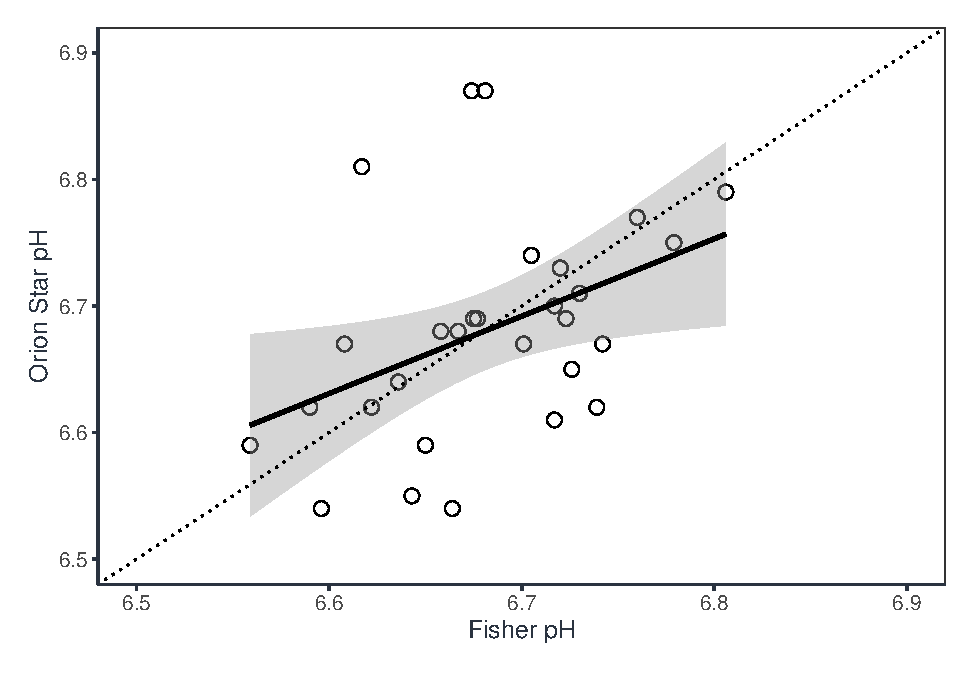
\includegraphics[width=0.5\textwidth]{ref_comparison.pdf}
  \caption{Comparison of pH results of reference sample measured with the Orion Star pH meter and with the Fisher Accumet pH meter ($\mbox{\textit{y}=0.44}$$\textit{x}$+$\mbox{4}$, $\mbox{\textit{n}=32}$, $\textit{R}$$^2$$\mbox{=0.05}$, $\mbox{\textit{p}> 0.01}$) from June 2023 to September 2023.}
\end{wrapfigure}

The pH results of reference samples were not well correlated among the
two pH meters (\emph{R\textsuperscript{2}} = 0.05,
\emph{p}\textgreater{} 0.01) with the pH measured on the Orion Star pH
meter ranging from 6.54 to 6.97 and the pH measured on the Fisher
Accumet pH meter ranging from 6.379 to 6.85.

\begin{wrapfigure}{r}{0.5\textwidth}
  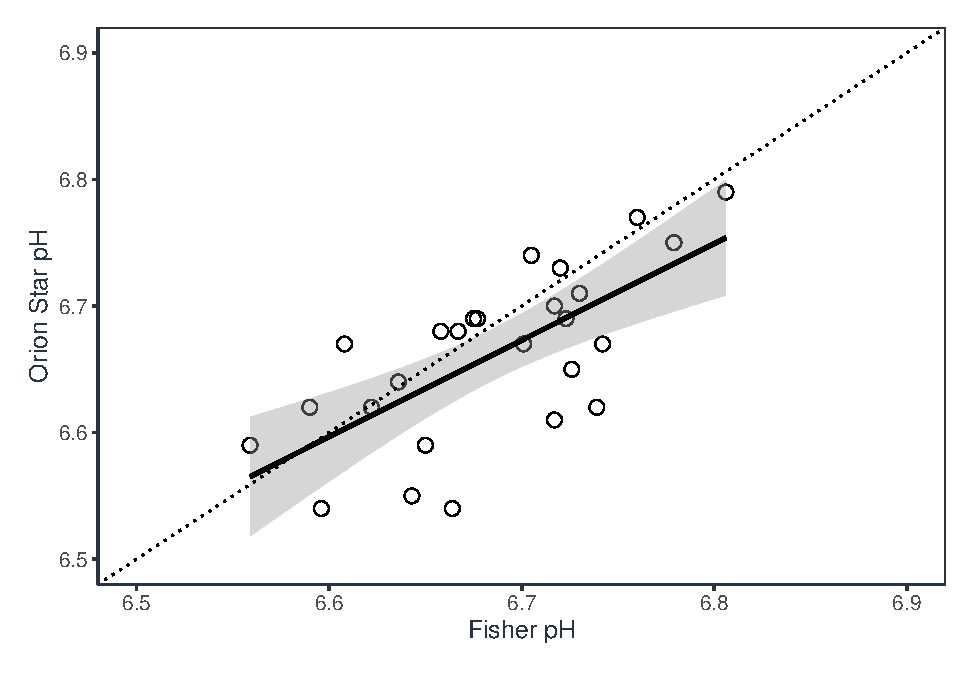
\includegraphics[width=0.5\textwidth]{ref_comparison_no_outliers.pdf}
  \caption{Comparison of pH results of reference sample measured with the Orion Star pH meter and with the Fisher Accumet pH meter from June 2023 to September 2023, with outliers (pH > 6.8) removed ($\mbox{\textit{y}=0.76}$$\textit{x}$+$\mbox{2}$, $\mbox{\textit{n}=26}$).}
\end{wrapfigure}

Five pH measurements of the reference sample using the Orion Star pH
meter were higher (pH \textgreater{} 6.8) than what would be expected by
the long-term trend (Figure 1 and Figure 2). These outliers did not
correspond to elevated analytical precision values or out of range
slopes. When these five outliers are removed, the correlation between pH
measured on the Orion Star pH meter and the Fisher Accumet pH meter is
improved (\emph{R\textsuperscript{2}} = 0.48) and is statistically
signficant (\emph{p} \textless{} 0.01. However, the slope (0.76)
indicates there is a bias, wherein the Fisher Accumet pH meter had
higher pH value than those witnessed on the Orion Star pH meter.

\pagebreak

\hypertarget{proficienty-testing-samples}{%
\subsection{Proficienty testing
samples}\label{proficienty-testing-samples}}

\hypertarget{comparison-with-fisher-accumet-ph-results}{%
\subsection{Comparison with Fisher Accumet pH
results}\label{comparison-with-fisher-accumet-ph-results}}

\begin{wrapfigure}{r}{0.5\textwidth}
  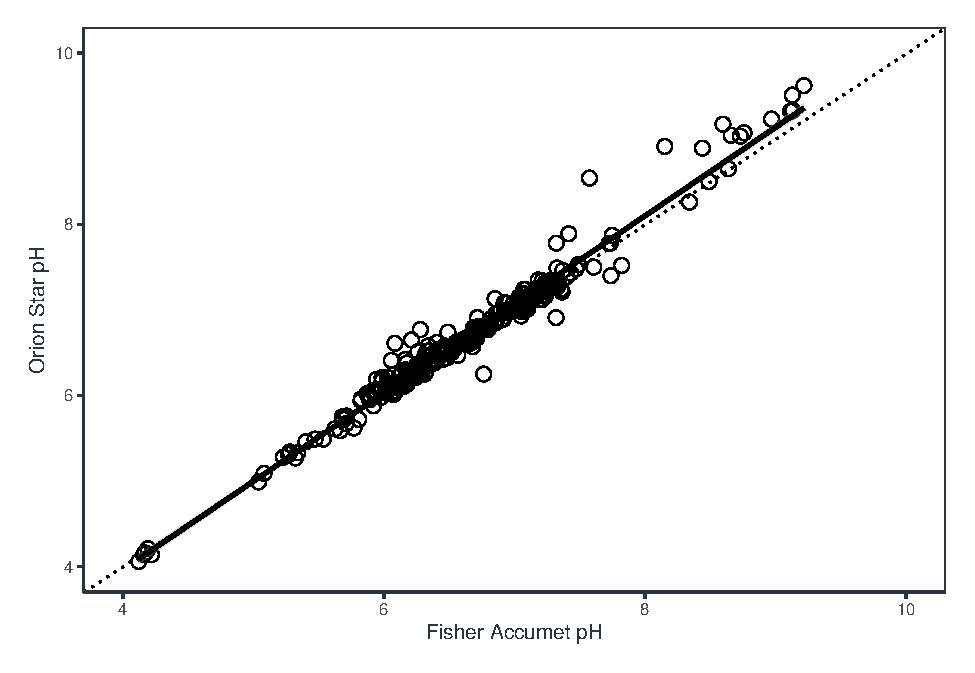
\includegraphics[width=0.5\textwidth]{fisher_v_orion.pdf}
  \caption{Comparison of pH results of samples measured on the Fisher Accumet pH meter and the Orion Star pH meter, $\mbox{\textit{y}=1.03}$$\textit{x}$$\mbox{-0.18}$, $\mbox{\textit{n}=301}$, $\textit{R}$$^2$$\mbox{=0.97}$, $\mbox{\textit{p}< 0.001}$.}
\end{wrapfigure}

Blah blah blah, just giving something for the figure to wrap around
until I write the text for this section.

\hypertarget{conclusions}{%
\subsection{Conclusions}\label{conclusions}}

\end{document}
